%! TeX program = xelatex
%! TEX-TS program = xelatex
\documentclass[twoside,9pt]{article}
\usepackage[left=1in, right=1in, top=1in, bottom=1in]{geometry}
\usepackage{amsmath}
\usepackage{amssymb}
\usepackage{amsfonts}
\usepackage{mathtools}
\usepackage{amsthm}
\usepackage{thmtools}
\usepackage{fancyhdr}
\usepackage{enumitem}
\usepackage{siunitx}
\usepackage{booktabs}
\usepackage[hidelinks]{hyperref}
\usepackage{sectsty}
\usepackage{mathrsfs} % mathscr
\usepackage{tikz}
\usepackage{tikz-3dplot}
\usepackage{pgfplots}
\usepackage{multicol}
\usepackage{listings}
% \usepackage{amsart}
\usepackage{fontspec}
\usepackage{soul}


% allow H option of figure
\usepackage{float}

% math font (libertine)
\usepackage{libertinus-otf}

% braket
\usepackage{braket}

% Chinese support
\usepackage{xeCJK}

% theorem colored box
\usepackage[many]{tcolorbox}

%% equation numbering
\numberwithin{equation}{section} % numbering equations by section
\renewcommand{\theequation}{\arabic{equation}} % remove section number

% tikz library
\usetikzlibrary{
    external,
    decorations,
    calc,
    3d,
}
\tikzexternalize[prefix=tikzpictures/]
\tikzexternaldisable
% input euler.tex, which includes tikz function for changing z-y-z to z-x-z
% Redefine the rotation sequence for the tikz3d-plot to Euler-Angles:
% z-x-z with alpha-beta-gamma (psi-theta-phi)
% https://tex.stackexchange.com/q/118069/98906
\newcommand{\tdseteulerzxz}{%
    \renewcommand{\tdplotcalctransformrotmain}{%
        %
        % Determine the sin and cos of the specified angle in degrees
        % \tdplotsinandcos{sin}{cos}{theta}
        % - #1: Returns sin(#3)
        % - #2: Returns cos(#3)
        % - #3: User-specified angle theta
        \tdplotsinandcos{\sinalpha}{\cosalpha}{\tdplotalpha} 
        \tdplotsinandcos{\sinbeta}{\cosbeta}{\tdplotbeta}
        \tdplotsinandcos{\singamma}{\cosgamma}{\tdplotgamma}
        %
        % Define trigonometric abbreviations
        %
        \tdplotmult{\sasb}{\sinalpha}{\sinbeta}
        \tdplotmult{\sacb}{\sinalpha}{\cosbeta}
        \tdplotmult{\sacbsg}{\sacb}{\singamma}
        \tdplotmult{\sacbcg}{\sacb}{\cosgamma}
        \tdplotmult{\sasg}{\sinalpha}{\singamma}
        \tdplotmult{\sacg}{\sinalpha}{\cosgamma}
        %
        \tdplotmult{\sbsg}{\sinbeta}{\singamma}
        \tdplotmult{\sbcg}{\sinbeta}{\cosgamma}
        %
        \tdplotmult{\casb}{\cosalpha}{\sinbeta}
        \tdplotmult{\cacb}{\cosalpha}{\cosbeta}
        \tdplotmult{\cacbsg}{\cacb}{\singamma}
        \tdplotmult{\cacbcg}{\cacb}{\cosgamma}
        \tdplotmult{\casg}{\cosalpha}{\singamma}
        \tdplotmult{\cacg}{\cosalpha}{\cosgamma}
        %
        % Define the entries for the rotation matrix from the B-System to the I-System
        % This is A_IB = (A_BI)^T
        %
        \pgfmathsetmacro{\raaeul}{+\cacg - \sacbsg}
        \pgfmathsetmacro{\rabeul}{-\casg - \sacbcg}
        \pgfmathsetmacro{\raceul}{+\sasb}
        %
        \pgfmathsetmacro{\rbaeul}{+\sacg + \cacbsg}
        \pgfmathsetmacro{\rbbeul}{-\sasg + \cacbcg}
        \pgfmathsetmacro{\rbceul}{-\casb}
        %
        \pgfmathsetmacro{\rcaeul}{+\sbsg}
        \pgfmathsetmacro{\rcbeul}{+\sbcg}
        \pgfmathsetmacro{\rcceul}{+\cosbeta}
        %
    }
}
 
% Redefine the rotation sequence for the tikz3d-plot to Cardan-Angles:
% x-y-z with alpha-beta-gamma
% https://tex.stackexchange.com/q/118069/98906
\newcommand{\tdsetcardanxyz}{%
    \renewcommand{\tdplotcalctransformrotmain}{%
        %
        % Determine the sin and cos of the specified angle in degrees
        % \tdplotsinandcos{sin}{cos}{theta}
        % - #1: Returns sin(#3)
        % - #2: Returns cos(#3)
        % - #3: User-specified angle theta
        \tdplotsinandcos{\sinalpha}{\cosalpha}{\tdplotalpha} 
        \tdplotsinandcos{\sinbeta}{\cosbeta}{\tdplotbeta}
        \tdplotsinandcos{\singamma}{\cosgamma}{\tdplotgamma}
        %
        % Define trigonometric abbreviations
        %
        \tdplotmult{\sasb}{\sinalpha}{\sinbeta}
        \tdplotmult{\sasbsg}{\sasb}{\singamma}
        \tdplotmult{\sasbcg}{\sasb}{\cosgamma}
        %
        \tdplotmult{\sacb}{\sinalpha}{\cosbeta}
        \tdplotmult{\sasg}{\sinalpha}{\singamma}
        \tdplotmult{\sacg}{\sinalpha}{\cosgamma}
        %
        \tdplotmult{\casb}{\cosalpha}{\sinbeta}
        \tdplotmult{\casbsg}{\casb}{\singamma}
        \tdplotmult{\casbcg}{\casb}{\cosgamma}
        %
        \tdplotmult{\cacb}{\cosalpha}{\cosbeta}
        \tdplotmult{\casg}{\cosalpha}{\singamma}
        \tdplotmult{\cacg}{\cosalpha}{\cosgamma}
        \tdplotmult{\cbsg}{\cosbeta}{\singamma}
        \tdplotmult{\cbcg}{\cosbeta}{\cosgamma}
        %
        % Define the entries for the rotation matrix from the B-System to the I-System
        % This is A_IB = (A_BI)^T
        %
        \pgfmathsetmacro{\raaeul}{+\cbcg}
        \pgfmathsetmacro{\rabeul}{-\cbsg}
        \pgfmathsetmacro{\raceul}{+\sinbeta}
        %
        \pgfmathsetmacro{\rbaeul}{+\casg + \sasbcg}
        \pgfmathsetmacro{\rbbeul}{+\cacg - \sasbsg}
        \pgfmathsetmacro{\rbceul}{-\sacb}
        %
        \pgfmathsetmacro{\rcaeul}{+\sasg - \casbcg}
        \pgfmathsetmacro{\rcbeul}{+\sacg + \casbsg}
        \pgfmathsetmacro{\rcceul}{+\cacb}
        %
    }
}


% physics
% \usepackage{physics}

% define latin modern font environment
\newcommand{\lms}{\fontfamily{lmss}\selectfont} % Latin Modern Roman
% \newcommand{\lmss}{\fontfamily{lmss}\selectfont} % Latin Modern Sans
% \newcommand{\lmss}{\fontfamily{lmtt}\selectfont} % Latin Modern Mono

% % change mathcal shape
% \usepackage[mathcal]{eucal}


% define math operators
\newcommand{\FF}{\mathbb{F}}
\newcommand{\RR}{\mathbb{R}}
\newcommand{\NN}{\mathbb{N}}
\newcommand{\ZZ}{\mathbb{Z}}
\newcommand{\QQ}{\mathbb{Q}}
\newcommand{\XX}{\mathbb{Y}}
\newcommand{\CL}{\mathcal{L}}
% \renewcommand{\d}{\mathrm{d}}
\renewcommand*\d{\mathop{}\!\mathrm{d}}
\DeclareMathOperator*{\argmax}{arg\,max}
\DeclareMathOperator*{\argmin}{arg\,min}
\DeclareMathOperator{\im}{im}
\DeclareMathOperator{\id}{id}
\DeclareMathOperator{\erf}{erf}
\renewcommand{\mod}[1]{\ (\mathrm{mod}\ #1)}

% section font style
\sectionfont{\lms\Large}
\subsectionfont{\lms\normalsize}
\subsubsectionfont{\bf}

% line spreading and break
\hyphenpenalty=5000
\tolerance=20
\setlength{\parindent}{0em}
\setlength\parskip{0.5em}
\allowdisplaybreaks
\linespread{0.9}

% enumerate settings
% no break before enumerate
\setlist[enumerate]{itemsep=2pt,topsep=2pt}
\setlist[itemize]{itemsep=2pt,topsep=2pt}

%%% theorem
%% amsthm theorem
% definition style
\theoremstyle{definition}
\newtheorem{theorem}{\lms Theorem}[section]
\newtheorem{axiom}{\lms Axiom}[section]
\newtheorem{definition}{\lms Definition}[section]
\newtheorem{example}{\lms Example}[section]
\newtheorem{question}{\lms Question}[section]
\newtheorem{exercise}{\lms Exercise}[section]
\newtheorem*{exercise*}{\lms Exercise}
\newtheorem{lemma}{\lms Lemma}[section]
\newtheorem{proposition}{\lms Proposition}[section]
\newtheorem{corollary}{\lms Corollary}[section]
\newtheorem*{theorem*}{\lms Theorem}
\newtheorem{problem}{\lms Problem}
% remark style
\theoremstyle{remark}
\newtheorem*{remark}{\lms Remark}
\newtheorem*{solution}{\lms Solution}
\newtheorem*{claim}{\lms Claim}

%% coloring theorem
% define colors
\colorlet{theoremcolor}{blue!4!white}
\colorlet{examplecolor}{gray!4!white}
\colorlet{definitioncolor}{green!3!white}
% theorem
\tcolorboxenvironment{theorem}{
  colback=theoremcolor,
  boxrule=0pt,
  boxsep=1pt,
  left=0pt,right=0pt,top=2pt,bottom=2pt,
  oversize=2pt,
  sharp corners,
  before skip=\topsep,
  after skip=\topsep,
  breakable,
}
% example
\tcolorboxenvironment{example}{
  colback=examplecolor,
  boxrule=0pt,
  boxsep=1pt,
  left=0pt,right=0pt,top=2pt,bottom=2pt,
  oversize=2pt,
  sharp corners,
  before skip=\topsep,
  after skip=\topsep,
  breakable,
}
% definition
\tcolorboxenvironment{definition}{
  colback=definitioncolor,
  boxrule=0pt,
  boxsep=1pt,
  left=0pt,right=0pt,top=2pt,bottom=2pt,
  oversize=2pt,
  sharp corners,
  before skip=\topsep,
  after skip=\topsep,
  breakable,
}


% paragraph indent
\setlength{\parindent}{0em}
\setlength\parskip{0.5em}

\newcommand\Code{PHY3110 SP23}
\newcommand\Ass{Notes}
\newcommand\name{Haoran Sun}
\newcommand\mail{haoransun@link.cuhk.edu.cn}

\title{{\lms \Code \ \Ass}}
\author{\lms \name \ (\href{mailto:\mail}{\mail})}
\date{\lms \today}

\makeatletter
% \let\Title\@title
\let\theauthor\@author
\let\thedate\@date

\fancypagestyle{plain}{%
    \fancyhf{}
    \lhead{\lms\Ass}
    \rhead{\lms\name}
    \rfoot{\lms\thepage}

    % # 页脚自定义
    \fancyfoot[L]{
        \begin{minipage}[c]{0.06\textwidth}
            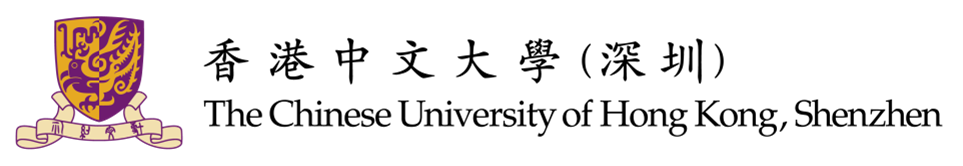
\includegraphics[height=7.5mm]{logo2.png}
        \end{minipage}
    }
}
\fancypagestyle{title}{%
    \fancyhf{}
    \renewcommand{\headrulewidth}{0pt}
    % \lhead{\Title}
    % \rhead{\theauthor}
    \rfoot{\lms\thepage}

    % # 页脚自定义
    \fancyfoot[L]{
        \begin{minipage}[c]{0.06\textwidth}
            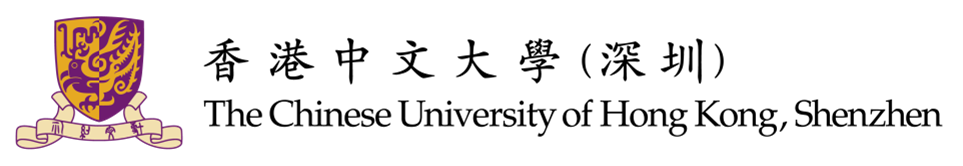
\includegraphics[height=7.5mm]{logo2.png}
        \end{minipage}
    }
}
\fancyfootoffset[L]{0.3cm}

% re-define title format
\makeatletter
\renewcommand{\maketitle}{\bgroup\setlength{\parindent}{0pt}
\begin{flushleft}
  \textbf{\Large\@title}

  \@author
\end{flushleft}\egroup
}
\makeatother

\pagestyle{plain}

% lstlisting settings
\lstset{
    basicstyle=\linespread{0.7}\footnotesize,
    breaklines=true,
    basewidth=0.5em
}


\begin{document}
\maketitle
\thispagestyle{title}
% \begin{multicols*}{2}

% \begin{remark}
%     $V_\epsilon(x)$ is used to denote a $\epsilon$-neighborhood
%     \begin{align*}
%         V_\epsilon(x) = B_\epsilon(x)\setminus\{x\}
%     \end{align*}
% \end{remark}

\tableofcontents
\newpage

\setcounter{section}{-1}
\section{Introduction}
\textbf{Grading:} 30\% homework, 30\% midterm, 40\% final.

\textbf{Textbooks:}
\begin{itemize}
    \item H. Goldstein, C. Poole, J. Safko, Classical Mechanics,
    3rd Edition, Pearson.
    \item J.R. Taylor, Classical Mechanics, University Science Books.
    \item T.W.B. Kibble, F.H. Berkshire, Classical Mechanics, 5th Edition,
    Imperial College Press.
    \item 梁昆淼,力学(下册)理论力学,4\textsuperscript{th} Edition,高等教育出版社.
\end{itemize}

Classical mechanics describe the motion of macroscopic objects, which are
not extremely massive and not extremely fast.

\section{Newtonian Mechanics}
Vectorial quantities of motion: position $\mathbf{r}$, 
velocity $\mathbf{v}$, force $\mathbf{F}$,
momentum $\mathbf{p}=m\mathbf{v}$,
angular momentum $\mathbf{L}=\mathbf{r}\times\mathbf{p}$.
Equations of motion are derived from those vector quantities.

Analytical mechanics uses scalar quantities of motion
\begin{itemize}
    \item Kinetic energy $T = \frac{1}{2}m\mathbf{v}^2$
    \item Potential energy $V = V(\mathbf{r})$
\end{itemize}
Equations of motion are derived from those scalar quantities.
\subsection{Newton's Laws}
\begin{theorem}[Newton's 2\textsuperscript{nd} law]
\begin{align}
    \mathbf{F} = \frac{\d \mathbf{p}}{\d t} = m\mathbf{a}
\end{align}
The formula is valid in an inertial frame.
\end{theorem}
Angular momentum $\mathbf{L}$ and torque $\mathbf{N}$ are also related
\begin{align}
    \frac{\d\mathbf{L}}{\d t} &= 
    \frac{\d}{\d t}(\mathbf{r}\times\mathbf{p})
    = \mathbf{r}\times\mathbf{F}
    = \mathbf{N}
\end{align}

Work done by external forces (note that $\d\mathbf{s}=\mathbf{v}\d t$)
\begin{align}
    W_{12} &= \int_1^2\mathbf{F}\d\mathbf{s}
    = \int_1^2 m\frac{\d\mathbf{v}}{\d t}\d\mathbf{s}
    = \int_1^2 m\mathbf{v}\d\mathbf{v}
    = \left.\frac{1}{2}m\mathbf{v}^2\right|_1^2
\end{align}

Define a scalar function $V(\mathbf{r})$,
then $\mathbf{F}=-\nabla V(\mathbf{r})$ is a conservative force.
\begin{align}
    \oint \mathbf{F}\d\mathbf{s} = 0
\end{align}

Center of mass of the system
\begin{align}
    \mathbf{R} &= 
    \frac{\sum_i m_i\mathbf{r}_i}{\sum_i m_i}
    =
    \frac{\sum_i m_i\mathbf{r}_i}{M}
\end{align}
Total momentum
\begin{align}
    \mathbf{P} 
    &= 
    \sum_i m_i\mathbf{p}_i
    = M\dot{\mathbf{R}}
\end{align}
Hence $\mathbf{P}$ is conserved if external force $\mathbf{F}^{(e)}$ is
zero.

Total angular momentum
\begin{align*}
    \frac{\d \mathbf{L}}{\d t} &= 
    \frac{\d }{\d t} \sum_i\mathbf{r}_i\times\mathbf{p}_i
    = \sum_i \mathbf{r}_i\times \left(
        \mathbf{F}_i^{(e)} + \sum_j \mathbf{F}_{ij}
    \right)
    = \sum_i\mathbf{r}_i\times\mathbf{F}_i^{(e)}
    + \sum_{ij}\mathbf{r}_i\times\mathbf{F}_{ij}
\end{align*}
Since $\mathbf{r}_{ij}$ parallel to $\mathbf{F}_ij$, then
\begin{align}
    \sum_{ij}\mathbf{r}_i\mathbf{F}_{ij} = 
    \frac{1}{2}\sum_{ij}\mathbf{r}_{ij}\times\mathbf{F}_{ji} = 0
\end{align}
Therefore
\begin{align}
    \frac{\d\mathbf{L}}{\d t} &= \mathbf{N}^{(e)}
\end{align}

Decomposition of the angular momentum
\begin{align}
    \mathbf{L} 
    &= \sum_i\mathbf{r}_i\times\mathbf{p}_i
    = \sum_i(\mathbf{R} + \mathbf{r}_i)\times m_i(\mathbf{V} + \mathbf{v}_i')
    = \sum_i \mathbf{R}\times m_i\mathbf{V}
    + \sum_i\mathbf{r}_i'\times m_i\mathbf{v}_i'
\end{align}

\subsection{Constraints}
Holonomic constraint
\begin{align}
    f(\mathbf{r}_1, \mathbf{r}_2, \dots, \mathbf{r}_N, t) &= 0
\end{align}
Example: rigid body
\begin{align}
    (\mathbf{r}_i-\mathbf{r}_j)^2 - c_{ij}^2 &= 0
\end{align}
Example: non-sliding cylinder
\begin{align*}
    \dot{x} - R\dot{\theta} = 0
    \Rightarrow x - R\theta = \text{const}
\end{align*}
A constraint of the form
\begin{align}
    \sum_i g_i(\mathbf{x}_1,\mathbf{x}_2,\dots,\mathbf{x}_n)\d\mathbf{x}_i = 0
    \Rightarrow
    \d G(\mathbf{x}_1,\dots) = 0
    \Rightarrow
    G(\mathbf{x}_1,\dots) = \text{const}
\end{align}

Non-holonomic constraint: cannot be written in the form of holonomic
constraint.

\subsection{Generalized coordinates}
Suppose we have a $N$-particle system, 
we will have $3N$ DOFs.
With $k$ constraints, we will have $3N-k$ DOFs.
Define $q_1,\dots,q_{3N-k}$ generalized coordinates,
we have
\begin{align}
    \mathbf{r}_i &= \mathbf{r}_i(q_1,\dots, q_{3N-1}, t)
\end{align}

\newpage
\section{Lagrange Formalism}
\subsection{D'Alembert's Principle}
Hint from the rigid body: internal forces of constraints do not work.

Virtual displacement: $\delta\mathbf{r}_i$
is consistent with the constraints imposed on the system at
a given time
\begin{align}
    \mathbf{r}_i \rightarrow 
    \mathbf{r}_i + \delta\mathbf{r}_i
\end{align}
\begin{theorem}[D'Alembert's principle]
Consider a system in equilibrium
\begin{align}
    \mathbf{F}_i = 0
    \Rightarrow
    \sum_i\mathbf{F}_i\cdot\delta\mathbf{r}_i = 0
\end{align}
Separate $\mathbf{F}_i = \mathbf{F}_i^{(a)} + \mathbf{f}_i$
where $\mathbf{f}_i$ is the constraint force.
Hence
\begin{align}
    \sum_i(\mathbf{F}_i^{(a)} + \mathbf{f}_i)
    \cdot\delta\mathbf{r}_i = 0
    \Rightarrow
    \sum_i\mathbf{F}_i^{(a)}\cdot\delta\mathbf{r}_i = 0
\end{align}
For a system moving under external forces
\begin{align}
    \mathbf{F}_i - \dot{\mathbf{p}}_i = 0
    \Rightarrow
    \sum_i(\mathbf{F}_i - \dot{\mathbf{p}}_i)\delta\mathbf{r}_i = 0
    \Rightarrow
    \sum_i(\mathbf{F}_i^{(a)} - \dot{\mathbf{p}}_i)\delta\mathbf{r}_i = 0
\end{align}
For holonomic constraints
\begin{align}
    \mathbf{r}_i = \mathbf{r}_i(q_1,\dots,q_n,t),\quad
    \mathbf{v}_i = \frac{\d\mathbf{r}_i}{\d t}
    = \frac{\partial \mathbf{r}_i}{\partial t}
    + \sum_j\frac{\partial\mathbf{r}_i}{\partial q_j}\dot{q}_j,\quad
    \delta\mathbf{r}_i = \sum_j\frac{\partial\mathbf{r}_i}{\partial q_j}
    \delta q_j
\end{align}
\end{theorem}
Define generalized force $Q_j$
\begin{align}
    \sum_i\mathbf{F}_i\delta\mathbf{r}_i
    &= \sum_{ij}\mathbf{F}_i\frac{\partial\mathbf{r}_i}{\partial q_j}\delta q_j
    = \sum_j Q_j\delta q_j
\end{align}
Then
\begin{align}
    \sum_i\dot{\mathbf{p}}_i\cdot\delta\mathbf{r}_i
    &= \sum_{ij}m_i\ddot{\mathbf{r}}_i
    \cdot\frac{\partial \mathbf{r}_i}{\partial q_j}\delta q_j
    = 
    \sum_{ij}\left[
        \frac{\d}{\d t}
        \left(m_i\dot{\mathbf{r}}_i\cdot\frac{\partial\mathbf{r}_i}{\partial q_j}\right)
        - m_i\dot{\mathbf{r}}_i\frac{\d}{\d t}\frac{\partial\mathbf{r}_i}{\partial q_j}
    \right]\delta q_j\\
    &= 
    \sum_j\left[
        \frac{\d }{\d t}\left(\frac{\partial T}{\partial\dot{q}_j}\right)
        - \frac{\partial T}{\partial q_j}
    \right]\delta q_j
    = \sum_j Q_j\delta q_j\\
\end{align}
where
\begin{align}
    \frac{\partial T}{\partial q_j}
    &= 
    \sum_{ik}\frac{\partial\dot\mathbf r_k}{\partial q_j}
    \frac{\partial}{\partial\dot\mathbf r_k} T
    = 
    \sum_k 
    m_k\dot\mathbf r_k
    \frac{\partial\dot\mathbf r_k}{\partial q_j}
    = 
    \sum_k 
    m_k\dot\mathbf r_k
    \frac{\d}{\d t}\frac{\partial\mathbf r_k}{\partial q_j}
\end{align}
Hence $\forall j$ we have
\begin{align}
    \frac{\d }{\d t}\left(\frac{\partial T}{\partial\dot{q}_j}\right)
    - \frac{\partial T}{\partial q_j}
    - Q_j = 0
    \label{lag0}
\end{align}
Let the potential energy $V=V(\mathbf{r}_i,\dots)=V(q_j,\dots)$,
then we have
\begin{align}
    Q_j &= \sum_i\mathbf{F}_i\frac{\partial\mathbf{r}_i}{\partial q_j}
    = \sum_i -\nabla_i V\frac{\partial\mathbf{r}_i}{\partial q_j}
    = -\frac{\partial V}{\partial q_j}
\end{align}
Therefore
\begin{align}
    \frac{\d }{\d t}\left(\frac{\partial (T-V)}{\partial\dot{q}_j}\right)
    - \frac{\partial (T-V)}{\partial q_j}
    - Q_j = 0
\end{align}
\begin{theorem}[Langrange's equation]
Define $L=T-V$, then
\begin{align}
    \frac{\d }{\d t}\left(\frac{\partial L}{\partial\dot{q}_j}\right)
    - \frac{\partial L}{\partial q_j}
    = 0
\end{align}
The choice of Lagrangian is not unique, $L'$ where
\begin{align}
    L' = L + \frac{\d F(q, t)}{\d t}
\end{align}
will give the same equations of motion as $L$.
\end{theorem}

\begin{example}[Lagrange's formalism]\
\begin{enumerate}[label=\arabic*)]
\item For a single particle moving under force $\mathbf{F}$
\begin{align*}
    L(\mathbf{x}, \dot{\mathbf{x}}, t) &= \frac{1}{2}m\dot{\mathbf{x}}^2 + \mathbf{F}\cdot\mathbf{x}
\end{align*}

\item Motion in a 2D plane using polar coordinates
\begin{align*}
    L(r, \theta, \dot{r}, \dot{\theta}, t) &= 
    \frac{1}{2}m(\dot{r}^2 + r^2\dot{\theta}^2)
    + F\cdot\mathbf{r}
\end{align*}
Generalized forces
\begin{align*}
    Q_r &= \mathbf{F}\cdot\frac{\partial\mathbf{r}}{\partial r}
    = \mathbf{F}\cdot\mathbf{e}_r\\
    Q_\theta &= \mathbf{F}\cdot\frac{\partial\mathbf{r}}{\partial\theta}
    = \mathbf{F}\cdot r\mathbf{e}_\theta
\end{align*}
where
\begin{align*}
    \mathbf{e}_r &= \begin{bmatrix}
        \cos\theta\\ \sin\theta
    \end{bmatrix}\quad
    \mathbf{e}_\theta = \begin{bmatrix}
        -\sin\theta\\ \cos\theta
    \end{bmatrix}
\end{align*}
Equations of motion
\begin{align*}
    m\ddot{r} - mr\dot{\theta}^2 &= \mathbf{F}\cdot\mathbf{e}_r\\
    mr^2\ddot{\theta} + 2mr\dot{r}\dot{\theta} &= r\mathbf{F}_\theta
\end{align*}

\item Atwood's machine
\begin{align*}
    L &= \frac{1}{2}(M_1+M_2)\dot{x}^2 + 
    M_1g x + M_2 g(l-x)
\end{align*}
The equation of motion is
\begin{align*}
    \frac{\d}{\d t}\frac{\partial L}{\partial \dot{x}}
    - \frac{\partial L}{\partial x} &= 0\\
    \Rightarrow (M_1 + M_2)\ddot{x} &= (M_1 - M_2)g
\end{align*}

\end{enumerate}
\end{example}

Suppose we have a potential dependent on velocity (generalized potential)
and the generalized force is defined as
\begin{align}
    U &= U(q_j,\dot{q}_j), \quad
    Q_j = -\frac{\partial U}{\partial q_j} 
    + \frac{\d }{\d t}\frac{\partial U}{\partial\dot{q}_j}
\end{align}
Define $L = T-U$, then we still have
\begin{align}
    \frac{\d }{\d t}\frac{\partial L}{\partial \dot{q}_j} - \frac{\partial L}{\partial q_j} &= 0
\end{align}
\begin{example}[Lorentz force on a moving charge]
The Lorentz force
\begin{align*}
    \mathbf{F} &= 
    q(\mathbf{E} + \mathbf{v}\times\mathbf{B})
\end{align*}
Define the scalar and vector potentials
\begin{align*}
    E &= -\nabla\phi - \frac{\partial \mathbf{A}}{\partial t},\quad
    \mathbf{B} = \nabla\times\mathbf{A}
\end{align*}
Hence
\begin{align*}
    \mathbf{F} &= 
    q\left[
        -\nabla\phi - \frac{\partial \mathbf{A}}{\partial t}
        + \mathbf{v}\times(\nabla\times\mathbf{A})
    \right]
\end{align*}

\end{example}

\subsection{Hamilton's principle, variational principle}
Configuration space: a space formed by the set of generalized coordinates.
\begin{align}
    (q_1, q_2, \dots, q_n)\text{ as function of $t$}
\end{align}
\begin{theorem}[Hamilton's principle]
Define the action integral $I$, where $L=T-V$ or $L=T-U$ ($U$ is the generalized
potential)
\begin{align}
    I =  \int_{t_1}^{t_2}L\d t
\end{align}
Then the variation of the action integral equals to zero
\begin{align}
    \delta I &= 
    \delta \int_{t_1}^{t_2}L(q_1,\dots, q_n,\dot{q}_1,\dots,\dot{q}_n)\d t
    = 0
\end{align}
Add small variation on the path
\begin{align}
    q_i(t, \alpha) &= q_i(t) + \alpha\eta(t)
\end{align}
where $\eta(t_1)=\eta(t_2)=0$.
Then the action will be the function of $\alpha$, $I=I(\alpha)$.
Hence
\begin{align}
    \delta I &= 
    \int_{t_1}^{t_2}\left(\sum_i \frac{\partial L}{\partial q_i}\delta q_i
    + \frac{\partial L}{\partial \dot{q}_i}\delta\dot{q}_i\right)\d t
\end{align}
Change the order of differentiation $\delta\dot{q}_i = \d \delta q_i/\d t$, then
\begin{align}
    \delta I(\alpha) &= 
    \int_{t_1}^{t_2}\sum_i\left[
        \frac{\partial L}{\partial q_i}\delta q_i
        - \frac{\d}{\d t}\left(\frac{\partial L}{\partial\dot{q}_i}\right)\delta q_i
        \right]\d t
        + \sum_i\frac{\partial L}{\partial\dot{q}_i}\delta q\large|_{t_1}^{t_2}\\
    &= 
    \int_{t_1}^{t_2}\sum_i\left[
        \frac{\partial L}{\partial q_i}
        - \frac{\d}{\d t}\left(\frac{\partial L}{\partial\dot{q}_i}\right)
    \right]\delta q_i\d t = 0 \\
    \Rightarrow
    & \frac{\d}{\d t}\left(\frac{\partial L}{\partial\dot{q}}\right)
    - \frac{\partial L}{\partial q_i} = 0
\end{align}
\end{theorem}

\begin{example}[Shortest path problem]
$y=y(x)$, $\d s = \sqrt{\d x^2 + \d y^2}$, then the action integral (path) is
\begin{align}
    I &= \int_1^2\d s = 
    \int_1^2\sqrt{1+\dot{y}^2}\d x
\end{align}
Apply the Lagrange's equation we get
\begin{align}
    \frac{\d }{\d x}\frac{\d \sqrt{1+\dot{y}^2}}{\d \dot{y}} = 0
    \Rightarrow \frac{\d\dot{y}}{\d x} = 0
    \Rightarrow y = ax + b
\end{align}
\end{example}

\begin{example}[Solid of revolution]
Differential of area $2\pi x\d s = 2\pi x\sqrt{1+\dot{y}^2}\d x$,
then the total area is
\begin{align}
    \int_1^2 2\pi x\sqrt{1+\dot{y}^2}\d x
\end{align}
Define the Lagrangian $L(x, y, \dot{y}) = 2\pi x\sqrt{1+\dot{y}^2}$,
by Lagrange's equation we can get
\begin{align}
    \frac{x\dot{y}}{\sqrt{1+\dot{y}^2}} = \text{const}
    \Rightarrow y = a\cosh^{-1}\frac{x}{a} + b
\end{align}
\end{example}

\begin{example}[The curve of fastest descent]
Question: along which trajectory from point 1 to point 2,
the time is shortest?
The total time is
\begin{align}
    T &= \int_1^2
    \frac{\d s}{v}
    = \int_1^2\frac{\d s}{\sqrt{2gy}}
\end{align}
According to Newton's laws we have $y=gv^2$, then
\begin{align}
    T &= \int_1^2\frac{\sqrt{1+\dot{y}^2}}{\sqrt{2gy}}\d x
\end{align}
Then we have $L(x, y, \dot{y})$ and we get
\begin{align}
    &2y\ddot y + 1 + \dot y^2 = 0\\
    \Rightarrow
    &2y\dot y\ddot y + \dot y + \dot y^3 
    = \dot y(1 + \dot y^2) + y (2\dot y\ddot y)
    = \frac{\d}{\d t}\dot y(1 + \dot y^2) = 0\\
    \Rightarrow
    &y(1 + \dot y^2) = \text{const}
\end{align}
which means that $y(1+\dot{y}^2)=\text{const}$.
The solution is $x=A(\theta-\sin\theta)$, $y=A(1-\cos\theta)$.
\end{example}

\subsection{Constraint}
Holonomic constraints
\begin{align}
    f(q_1,\dots,q_n,t) &= 0
\end{align}
Non-holonomic constraints
\begin{align}
    f(q_1,\dots,q_n;\dot{q}_1,\dots,\dot{q}_n;t) &= 0
\end{align}
Sometimes we can convert $f(\dot{q}_i)=0$ to $f'(q_i)=0$.
\begin{example}[Rolling cylinder]
Rolling cylinder without sliding has the constraint
\begin{align}
    \dot{x} - R\dot{\theta} = 0
    \Rightarrow x-R\theta = \text{const}
\end{align}
\tikzexternalenable
\begin{figure}[H]
    \centering
    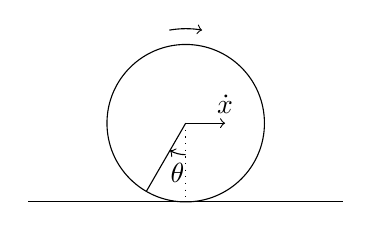
\begin{tikzpicture}
        \draw (-2,0)--(2,0);
        \draw (0,1) circle (1);
        \draw[->] (0,1)+(100:1.2) arc (100:80:1.2);
        \draw[->] (0,1) -- (0.5, 1) node[above] {$\dot x$};
        \draw[dotted] (0, 1) -- (0,0);
        \draw (0, 1) --++ ({cos(-120)},{sin(-120)});
        \draw[->] (0, 0.6) arc (-90:-120:0.4) node[midway,below] {$\theta$};
    \end{tikzpicture}
\end{figure}
\tikzexternaldisable
\end{example}

A commonly encountered type of non-holonomic constraint is linear constraint equations
\begin{align}
    \sum_{k=1}^n a_{ik}\frac{\d q_k}{\d t} + a_i t &= 0
\end{align}
For the virtual displacement $\delta q_i$
\begin{align}
    \sum_{k=1}^n a_{ik}\delta q_k &= 0
\end{align}

Suppose $q_i$ are not independent, then the Euler-Lagrange's equation
could not hold.
\begin{align*}
    \int_{t_1}^{t_2}\sum_i\left[
        \frac{\partial L}{\partial q_i}
        - \frac{\d}{\d t}\left(\frac{\partial L}{\partial\dot{q}_i}\right)
    \right]\delta q_i\d t = 0 
    \nRightarrow
    \frac{\d}{\d t}\left(\frac{\partial L}{\partial\dot{q}}\right)
    - \frac{\partial L}{\partial q_i} = 0
\end{align*}
Include the constraint equation of $q_i$ into the equation
\begin{align}
    \sum_{k=1}^n a_{ik}\delta q_k &= 0
    \Rightarrow
    \sum_{i=1}^m \lambda_i\sum_{k=1}^n a_{ik}\delta q_k = 0
\end{align}
Hence
\begin{align*}
    \int_{t_1}^{t_2}\sum_{k=1}^n\left[
        \frac{\partial L}{\partial q_k}
        - \frac{\d}{\d t}\left(\frac{\partial L}{\partial\dot{q}_k}\right)
        + \sum_{i=1}^m\lambda_i a_{ik}
    \right]\delta q_k\d t = 0 
\end{align*}
Let $q_1,\dots,q_{n-m}$ be independent generalized coordinate,
$q_{n-m+1},\dots,q_n$ dependent generalized coordinates (i.e., they can
be expressed by $q_1,\dots,q_{n-m}$).
Choose $\lambda_i$ s.t.
\begin{align}
    \frac{\partial L}{\partial q_k}
    - \frac{\d}{\d t}\left(\frac{\partial L}{\partial\dot{q}_k}\right)
    + \sum_{i=1}^m\lambda_i a_{ik}
    = 0
\end{align}
$\forall k = n-m+1,\dots,n$.
In conclusion, we have $q_1,\dots,q_n,\lambda_1,\dots,\lambda_m$ overall
$n+m$ unknowns, and $n$ Lagrange's equations and $m$ constraint equations
overall $n+m$ equations.
\begin{remark}\ 
\begin{enumerate}[label=\arabic*)]
\item It is inconvenient to reduce all $q_k$s to independent 
coordinates
\item If we are interested in the constraint forces
\begin{align*}
    \sum_{k=1}^n a_{ik}\d q_k + a_{it}\d t = 0
\end{align*}
where 
\begin{align*}
    a_{ik} &= \frac{\partial f_i}{\partial q_k},\quad
    a_{it} = \frac{\partial f_i}{\partial t}
\end{align*}
Then
\begin{align*}
    \d f_i &= \frac{\partial f_i}{\partial q_k}\d q_k + 
    \frac{\partial f_i}{\partial t}\d t
    \Rightarrow \d f_i = 0,~f_i=\text{const}
\end{align*}
\end{enumerate}
\end{remark}

\begin{example}[Hoop rooling down an inclined plane]\
\tikzexternalenable
\begin{figure}[H]
    \centering
    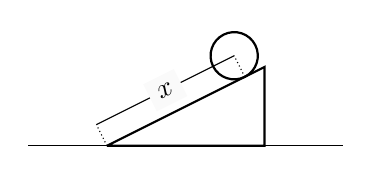
\begin{tikzpicture}
        \draw (0,0)--(4,0);
        \draw[thick] (1,0) -- (3,0) -- (3,1) -- (1,0);
        \draw[thick] (2.75,0.875) arc ({-atan(2)}:{360-atan(2)}:0.3);
        \draw[densely dotted] (2.75,0.875) --++ ({180-atan(2)}:0.3);
        \draw[densely dotted] (1,0) --++ ({180-atan(2)}:0.3);
        \draw ($ (2.75,0.875) + ({180-atan(2)}:0.3) $) -- 
              node[midway,sloped,fill=examplecolor] {$x$}
              ($ (1,0) + ({180-atan(2)}:0.3) $);
    \end{tikzpicture}
\end{figure}
\tikzexternaldisable
The constraint equation writes
\begin{align*}
    \dot{x} - r\dot{\theta} = 0
    \Rightarrow x - r\theta = \text{const}
\end{align*}
$a_x=1$, $a_\theta = -r$, $a_t=0$.

Energy terms are
\begin{align*}
    T &= 
    T_\text{COM} + T_\text{relative}
    = \frac{1}{2}M\dot{x}^2 + \frac{1}{2}M(r\dot{\theta})^2\\
    V &= Mg(l-x)\sin\phi\\
    \Rightarrow
    L &=  \frac{1}{2}M\dot{x}^2 + \frac{1}{2}M(r\dot{\theta})^2
    - Mg(l-x)\sin\phi
\end{align*}
Then we can write the Lagrange's equation with Lagrange's multipliers
\begin{align*}
    \frac{\partial L}{\partial x} - \frac{\d }{\d t}\frac{\partial L}{\partial \dot{x}}
    + a_x\lambda &= 0\\
    \Rightarrow
    Mg\sin\phi - M\ddot{x} + \lambda &= 0\\
    -Mr^2\ddot{\theta} - \lambda r &= 0\\
    \dot{x} &= r\dot{\theta}\Rightarrow
    \ddot{x} = r\ddot{\theta}
\end{align*}
we can get $M\ddot{x} = Mr\ddot{\theta} = -\lambda$ and 
$\ddot{x} = (g\sin\phi)/2$.
Note that $\lambda$ is the constraint force (in this case $\lambda$
is the frictional force).
\end{example}

\subsection{Lagrangian for Lorentz force}
The Lorentz force is given by
\begin{align}
    \mathbf{F} &= 
    q[\mathbf{E} + \mathbf{v}\times\mathbf{B}]
    \label{eq-EMEOM}
\end{align}
Where
\begin{align}
    \mathbf{E} &= -\nabla\phi - \frac{\partial A}{\partial t},\enskip
    \mathbf{B} = \nabla\times\mathbf{A}
\end{align}
Hence, by defining the Lagrangian
\begin{align}
    L &= 
    \frac{1}{2}m\mathbf{v}^2 - q\phi + q\mathbf{A}\cdot\mathbf{v}
\end{align}
Applying the Lagrange's equation we can get the EOM (eq. \ref{eq-EMEOM}).
Take $x$ as an example
\begin{align}
    \frac{\d}{\d t}\frac{\partial L}{\partial \dot x}
    &= \frac{\d}{\d t}(m\dot x + qA_x)
    = m\ddot x + q\frac{\partial A_x}{\partial t} + \mathbf{v}\cdot\nabla A_x
\end{align}

\subsection{Conservation \& symmetry of the system}
\begin{definition}[Cylic coordinate]
The generalized coordinate $q_i$ is cyclic (ignorable) if 
\begin{align}
    \frac{\partial L}{\partial q_i} &= 0
\end{align}
It implies the generalized momentum $p_i$ is conserved.
\end{definition}
\textbf{Rotational symmetry.}
Let $q_j$ be one of the rotational angle of spacial coordinate $\mathbf{r}_i$.
Hence
\begin{align}
    \d\mathbf{r}_i &= 
    \mathbf{n}_j\times\mathbf{r}_i\d q_j
    \Rightarrow
    \frac{\partial\mathbf{r}_i}{\partial q_j} = 
    \mathbf{n}_j\times\mathbf{r}_i\d q_j
\end{align}
where $\mathbf{n}_j$ is the normal vector of the rotation axis of $q_j$.
Hence the generalized force of $q_j$ writes
\begin{align}
    Q_{q_j} &= -\frac{\partial V}{\partial q_j} = 
    -\sum_k\frac{\partial V}{\partial\mathbf{r}_k}\frac{\partial\mathbf{r}_k}{\partial q_j}
    = -\frac{\partial V}{\partial\mathbf{r}_i}\frac{\partial\mathbf{r}_i}{\partial q_j}
    = \mathbf{F}_i\cdot(\mathbf{n}_j\times\mathbf{r}_i)
    = \mathbf{n}_j\cdot(\mathbf{r}_i\times\mathbf{F}_i)
    = \mathbf{n}_j\cdot\mathbf{N}_i
\end{align}
where $\mathbf{N}_i$ stands for the torque on the $i$\textsuperscript{th} particle.
The generalized momentum of $q_j$ writes
\begin{align}
    p_{q_j} &=
    \frac{\partial T}{\partial\dot{q}_j}
    = \sum_k\frac{\partial T}{\partial\dot\mathbf{r}_k}\frac{\partial\mathbf{r}_i}{\partial q_j}
    = \sum_k m_k\dot\mathbf{r}_k\cdot\frac{\partial\dot\mathbf{r}_k}{\partial\dot q_j}
    = m_i\dot\mathbf{r}_i\cdot(\mathbf{n}_j\times\mathbf{r}_i)
    = \mathbf{n}_j\times (\mathbf{r}_i\times m_i\dot\mathbf{r}_i)
    = \mathbf{r}_j\times\mathbf{L}_i
\end{align}
where $\mathbf{L}_i$ stands for the angular momentum of the $i$\textsuperscript{th} particle.
Hence, the rotational invariance implies the conservation of angular momentum.

\textbf{Time translation}
\begin{align}
    \frac{\d}{\d t}L &= 
    \sum_i\frac{\partial L}{\partial q_i}\dot{q}_i
    + \frac{\partial L}{\partial \dot{q}_i}\ddot{q}_i
    + \frac{\partial L}{\partial t}\\
    &= \sum_i\frac{\d}{\d t}\frac{\partial L}{\partial\dot{q}_i}\dot{q}_i
    + \frac{\partial L}{\partial \dot{q}_i}\ddot{q}_i
    + \frac{\partial L}{\partial t}\\
    &= \frac{\d}{\d t}\sum_i\left(\frac{\partial L}{\partial\dot{q}_i}\dot{q}_i\right)
    + \frac{\partial L}{\partial t}\\
    \Rightarrow &
    \frac{\partial L}{\partial t} + 
    \frac{\d}{\d t}\underbrace{\left(
    \sum\frac{\partial L}{\partial\dot{q}_i}q_i - L
    \right)}_{H}
    = 0
\end{align}
Note that
\begin{align}
    \sum_i\frac{\partial L}{\partial\dot{q}_i}\dot{q}_i &= 2T
\end{align}
\begin{proof}
Suppose $r_i$ does not have explicit time dependence ($\partial r_i/\partial t=0$)
\begin{align*}
    T &= \sum_i \frac{1}{2}m_i\dot{r}_i^2
    = \sum_i \frac{1}{2}m_i\left(
        \sum_j\frac{\partial r_i}{\partial q_j}\dot{q}_j
        + \frac{\partial r_i}{\partial t}
    \right)^2\\
    &= \sum_{ijk}
    \frac{1}{2}m_i\frac{\partial r_i}{\partial q_j}
    \frac{\partial r_i}{\partial q_k}\dot{q}_j\dot{q}_k\\
    \Rightarrow
    \sum_i\frac{\partial L}{\partial\dot{q}_i}\dot{q}_i
    &= 
    \sum_i \dot{q}_i \sum_{jk}
    m_k\frac{\partial r_k}{\partial q_i}\frac{\partial r_k}{\partial q_j}
    \dot{q}_j 
    = \sum_{ijk}
    m_k\frac{\partial r_k}{\partial q_i}\frac{\partial r_k}{\partial q_j}
    \dot q_i \dot{q}_j
    = 2T\qedhere
\end{align*}
\end{proof}
Hence we can define Hamiltonian $H = T+V$ which stands for the total energy,
and $H$ conserved if $L$ doesn't depend on time explicitly.

\begin{example}[Two blocks]\
Let $M$ be the mass of the big block,
$m$ be the mass of the small block.
Define two generalized coordinates:
$X$ stand for the position of COM of the big block,
$q$ stand for the position of COM of the small block
(sloped). 
\tikzexternalenable
\begin{figure}[H]
    \centering
    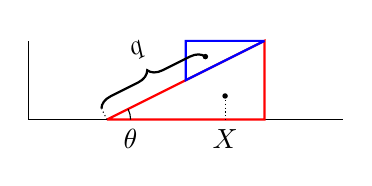
\begin{tikzpicture}
        \draw (0,0)--(4,0);
        \draw (0,0)--(0,1);
        \draw[red,thick] (1,0)--(3,0)--(3,1)--(1,0);    % large block
        \draw[blue,thick] (3,1)--(2,1)--(2,0.5)--(3,1); % small block
        \node[circle,fill,inner sep=0.7pt] at (2.5,0.3) {}; % COM large block
        \node[circle,fill,inner sep=0.7pt] at (2.25,0.8) {}; % COM small block
        \draw[densely dotted] (2.5,0.3)--(2.5,0) node[below,text opacity=1] {$X$}; % X label
        \draw (1,0)+(0:0.3) node[below] {$\theta$} arc (0:atan(1/2):0.3); % theta helper line
        \draw[densely dotted] (1,0)--++ ({180 - atan(2)}:0.15652); % q helper line (left)
        \draw[thick,decorate,decoration={brace,amplitude=5pt}]
            ($ (1,0)+({180-atan(2)}:0.15652) $) -- node[midway,sloped,above=6pt] {$q$} (2.25,0.8); % q brace
    \end{tikzpicture}
\end{figure}
\tikzexternaldisable
Hence we can easily define the Lagrangian
\begin{align*}
    L &= 
    \frac{1}{2}M\dot{X}^2
    + \frac{1}{2}m[
        (\dot{X} + \dot{q}\cos\theta)^2
        + \dot{q}^2\sin^2\theta
    ] - mgq\sin\theta
\end{align*}
There is no $X$ dependence on the system, hence
$X$ is a cyclic coordinate.
\begin{align*}
    \frac{\d}{\d t}\frac{\partial L}{\partial\dot{X}}
    &= \frac{\d}{\d t}M\dot{X} + m(\dot{X} + \dot{q}\cos\theta) = 0\\
    \Rightarrow &M\dot{X} m(\dot{X} +\dot{q}\cos\theta) = p_X = \text{const}
\end{align*}
\end{example}


\newpage
\section{The Central Force Problem}
\subsection{Reduction to the equivalent one-body problem}
For the two-body problem, we have two choices of
generalized coordinate
\begin{enumerate}[label=(\alph*)]
    \item $\mathbf{r}_1$, $\mathbf{r}_2$ stand for spacial coordinates of two
    masses
    \item $\mathbf{R}$ spacial coordinate of the COM, $\mathbf{r}=\mathbf{r}_1-\mathbf{r}_2$
\end{enumerate}
Hence, we can rewrite the kinetic energy in terms of $\mathbf{R}$ and $\mathbf{r}$
\begin{align}
    T &= \frac{1}{2}m_1\dot\mathbf{r}_1^2 + \frac{1}{2}m_2\dot\mathbf{r}_2^2\\
    &= \frac{1}{2}m_1\left(\dot\mathbf{R}+\frac{m_2}{m_1+m_2}\dot\mathbf{r}\right)^2
    + \frac{1}{2}m_2\left(\dot\mathbf{R}-\frac{m_1}{m_1+m_2}\dot\mathbf{r}\right)^2\\
    &= \frac{1}{2}(m_1+m_2)\dot\mathbf{R}^2 + \frac{m_1m_2}{m_1+m_2}\dot\mathbf{r}^2
    = \frac{1}{2}M\dot\mathbf{R}^2 + \frac{1}{2}\mu\dot\mathbf{r}^2
\end{align}
Hence we can write the Lagrangian
\begin{align}
    L &= 
    \frac{1}{2}M\dot\mathbf{R}^2 + \frac{1}{2}\mu\dot\mathbf{r}^2 - V
\end{align}
Suppose $V=V(\mathbf{r})$, then $\mathbf{R}$ is a cyclic coordinate,
We have $\dot\mathbf{R}=\text{const}$, and we can drop $\dot{\mathbf{R}}$
terms in $L$.
Moreover, if $V=V(\|\mathbf{r}\|)$, the total angular momentum is conserved.

Use $r$, $\theta$ as generalized coordinates, we have
\begin{align}
    L &= \frac{1}{2}\mu(\dot{r}^2 + r^2\dot{\theta}^2) - V(r)
\end{align}
The Lagrange's equation wrt $r$ writes
\begin{align}
    \mu\ddot{r}
    - \mu r\dot{\theta}^2
    + \frac{\partial V}{\partial r} &= 0
\end{align}
Easy to find that $\theta$ is cyclic, hence
\begin{align}
    \frac{\d}{\d t}\frac{\partial L}{\partial\dot\theta}
    &= \frac{\d}{\d t}\mu r^2\dot\theta = 0
    \Rightarrow p_\theta = \mu r^2\dot{\theta} = l = \text{const}
\end{align}
\begin{theorem}[Kepler's 2\textsuperscript{nd} law]
Radius vector sweeps out equal areas in equal time.
\end{theorem}
Substitute $\mu r\dot{\theta}^2$ term by $L$, we have
\begin{align}
    &\mu\ddot{r} - \frac{l^2}{\mu r^3} + \frac{\partial V}{\partial r} = 0\\
    \Rightarrow
    &\mu\ddot{r} = -\frac{\partial}{\partial r}(V + \frac{l^2}{2\mu r^2})\\
    &\mu\ddot{r}\dot{r} = -\frac{\partial}{\partial r} \dot{r}(V + \frac{l^2}{2\mu r^2})\\
    \Rightarrow
    &\frac{\d}{\d t}(\frac{1}{2}\mu\dot{r}^2 + V + \frac{l^2}{2\mu r^2}) = 
    \frac{\d }{\d t}E = 0
\end{align}
Hence we can get the expression of $\dot{r}$
and a differential equation
\begin{align}
    \dot{r} &= 
    \sqrt{
        \frac{2}{\mu}(E - V - \frac{l^2}{2\mu r^2})
    }
\end{align}
Define the new effective force $f'(r)$ with an 
effective potential $V'= V + l^2/2\mu r^2$, we have
\begin{align}
    \mu\ddot{r} &= 
    -\frac{\partial V}{\partial r} + \frac{l^2}{\mu r^3} 
    = f'(r),\quad
    E = \frac{1}{2}\mu\dot{r}^2 + V' = \text{const}
\end{align}
\begin{example}[Gravitational force]
Suppose we have $f(r) = -kr^{-2}$ and $V=-kr^{-1}$, then
\begin{align*}
    V' &= -\frac{k}{r} + \frac{l^2}{2\mu r^2}
\end{align*}
\tikzexternalenable
\begin{figure}[H]
    \centering
    \begin{tikzpicture}
        \draw[->] (0, 0) -- (4,0) node[below,xshift=4pt] {$r$};
        \draw[->] (0, -1) -- (0, 2) node[left] {$V'$};
        \draw[domain=0.12:4,variable=\x,smooth,samples=500]
            plot ({\x}, {0.1*(1/\x^2 - 6/\x)});
        \draw[dashed] (0, -0.4) node[left] {$E$} -- (2, -0.4);
        \draw[densely dotted] (0.1910, -0.4) -- (0.1910, 0) node[above,xshift=4pt] {$r_1$};
        \draw[densely dotted] (1.3090, -0.4) -- (1.3090, 0) node[above] {$r_2$};
    \end{tikzpicture}
\end{figure}
\tikzexternaldisable
\begin{enumerate}[label=\arabic*)]
    \item $E=E_1\geq 0$, the motion has a lower bound, $r\geq r_1$.
    \item $V_\text{min} < E_2 < 0$, the motion has lower and upper bound,
    $r_1\leq r \leq r_2$.
    \item $E_3 = V_\text{min}$, the motion will shrink to a single circle
    $r_1 = r_2 = \text{const}$, hence it is a circular motion.
    In this case, the gravitational force is equal to the centrifugal
    force
    \begin{align*}
        \mu\ddot{r} &= f(r) + \frac{l^2}{\mu r^3}
        = f(r) + \mu r\dot{\theta}^2 = 0
        \Rightarrow
        f(r) = -\mu r\dot{\theta}^2
    \end{align*}
\end{enumerate}
\begin{remark}
Let the potential be $V=-kr^{-\alpha}$,
then the motion cannot have periodic behavior if $\alpha>2$.
\end{remark}
\end{example}

\begin{example}[Harmonic oscillator]
$V=kr^2/2$, we have
\begin{align*}
    V' &= \frac{1}{2}kr^2 + \frac{l^2}{2\mu r^2}
\end{align*}
\end{example}

\begin{theorem}[Conditions for closed orbitals, Bertrand's theorem]
Stable orbitals require
\begin{align}
    \left.\frac{\partial^2 V'}{\partial r^2}\right|_{r=r_0}
    &= \left.-\frac{\partial f}{\partial r} + \frac{3l^2}{mr^4} \right|_{r=r_0}>0
    \Rightarrow
    \left.\frac{\partial f}{\partial r}\right|_{r=r_0} < -\frac{3f(r_0)}{r_0}
\end{align}
Let $f=-kr^n$, then we have
\begin{align}
    -knr^{n-1} &< 3kr^{n-1}
    \Rightarrow
    n > -3
\end{align}
For a small perturbation from the minimum, we can write the effective potential
as Taylor expansion
\begin{align}
    V'(r) &= 
    V'(r_0) + \left.\frac{\partial V'}{\partial r}\right|_{r=r_0}(r-r_0)
    + \frac{1}{2}\left.\frac{\partial^2 V'}{\partial r^2}\right|_{r=r_0}
    (r-r_0)^2 + \cdots \\
    & = V'(r_0) + \frac{1}{2}\left.\frac{\partial^2 V'}{\partial r^2}\right|_{r=r_0}
    (r-r_0)^2 + O(|r-r_0|^3)
\end{align}
Hence the EOM becomes 
\begin{align}
    m\ddot{r} &= -\frac{\partial V'}{\partial r}
    = \left.-\frac{\partial^2 V'}{\partial r^2}\right|_{r=r_0}(r-r_0)\\
    \dot\theta &= \frac{l}{mr^2}
\end{align}
The solution taks the form
\begin{align}
    u &= u_0 + a\cos \beta\theta, ~u=\frac{1}{r},~
    \beta^2 = \left.\frac{r}{f}\frac{\partial f}{\partial r} + 3\right|_{r=r_0}
\end{align}
For finite perturbation, the orbit can be a closed only if $\beta^2=1$ or $4$.
Then there are only two types of central-force scalar problem with the property
that all bound orbitals are closed orbitals.
\begin{align}
    \left.\frac{r}{f}\frac{\partial f}{\partial r}\right|_{r=r_0} 
    &= \pm 2\Rightarrow
    f = -kr^{-2}\text{ or } -kr
\end{align}

\hl{check the theorem on other books}
\end{theorem}

\subsection{Virial theorem}
Consider a multi-particle system $1\leq i\leq N$.
\begin{align}
    \dot \mathbf{p}_i &= \mathbf{F}_i
\end{align}
Define new function 
\begin{align}
    G &= \sum_i \mathbf{p}_i\cdot\mathbf{r}_i
\end{align}
Then the time derivative of $G$ writes
\begin{align}
    \frac{\d}{\d t}G &= 
    \sum_i m_i\dot \mathbf{r}_i^2 + \sum_i \mathbf{F}_i\cdot\mathbf{r}_i
\end{align}
Hence the time average of $\d G/\d t$ is
\begin{align}
    \frac{1}{\tau}\int_0^\tau \frac{\d}{\d t}G \d t
    &= 2\overline{T} + \overline{\sum_i\mathbf{F}_i\cdot\mathbf{r}_i}
    = \frac{1}{\tau}[G(\tau) - G(0)]
\end{align}
The time average equals to $0$ if $\tau$ is the period of the periodic motion;
even for non-periodic motion, if $\tau\rightarrow\infty$, the average will
approach $0$.
Hence
\begin{align}
    2\overline{T} + \overline{\sum_i\mathbf{F}_i\cdot\mathbf{r}_i} &= 0
    \Rightarrow
    \overline{T} = -\frac{1}{2}
    \underbrace{
        \overline{\sum_i\mathbf{F}_i\cdot\mathbf{r}_i}
    }_{\mathclap{\text{virial of Clausius}}}
    \label{eq:virial1}
\end{align}

\begin{example}[Ideal gas]
Temperature $T\propto T_i$ kinetic energy of $i$\textsuperscript{th}
particle.
\begin{align}
    T_i &= \frac{3}{2}k_BT
\end{align}
Hence the time average of total kinetic energy is
\begin{align}
    \overline{\sum_i T_i} &= 
    \frac{3}{2}Nk_BT
\end{align}
The virial could be written as
\begin{align}
    \overline{\sum_i\mathbf{F}_i\cdot\mathbf{r}_i} &= 
    \int\d\mathbf{F}\cdot\mathbf{r}
\end{align}
Note that
\begin{align*}
    \d\mathbf{F} &= -p\d A\mathbf{n}
\end{align*}
Applying Gauss's law we have
\begin{align}
    \overline{\sum_i\mathbf{F}_i\cdot\mathbf{r}_i} &= 
    -\int p\d A\ \mathbf{n}\cdot\mathbf{r}
    = -\int p\d V\ (\nabla\mathbf{r})
    = -3pV
\end{align}
Hence by the equation we get $pV=nk_BT$.
\end{example}

\begin{example}[Gravational force]
Since $\mathbf{F}_i =-\nabla_i V$, 
given $V_i=ar_i^{n+1}$, we have
\begin{align}
    \overline{T} &= 
    \frac{1}{2}\overline{\sum_i\nabla_i V\cdot\mathbf{r}_i}
    = \frac{n+1}{2}\overline{\sum_i a r_i^{n+1}}
    = \frac{n+1}{2}\overline{V}
\end{align}
\end{example}

This theorem is particularly important when the potential energy is a homogeneous
function of the coordinates, i.e.
\begin{align}
    U(\alpha\mathbf{r}_1, \dots, \alpha\mathbf{r}_n) &=
    \alpha^k
    U(\mathbf{r}_1, \dots, \mathbf{r}_n)
\end{align}
Note that
\begin{align}
    \frac{\d U}{\d \alpha}
    &= 
    \sum_a \frac{\partial \alpha \mathbf{r}_a}{\partial \alpha}\cdot\frac{\partial U}{\partial \alpha\mathbf{r}_a}
    = 
    \sum_a \frac{\mathbf{r}_a}{\alpha} \cdot\frac{\partial U}{\partial \mathbf{r}_a}
    = k\alpha^{k-1} U
\end{align}
Then the equation \ref{eq:virial1} becomes
\begin{align}
    2\overline{T} &= k\overline{U}
\end{align}
Equivalently
\begin{align}
    \overline{U} &= \frac{2E}{k + 2},~
    \overline{T}  = \frac{kE}{k + 2}
\end{align}

\subsection{Inverse-square force}
Consider $f=-k/r^2$, $V=-k/r$,
then we have EOM
\begin{align}
    \dot r &= \left[
        \frac{2}{m}\left(E + \frac{k}{r} - \frac{l^2}{2mr^2}\right)
    \right]^{1/2}
    \Rightarrow
    \theta = \theta_0 + \int_{r_0}^{r_1}\frac{\d r}{r^2\left(
        \frac{2mE}{l^2} - \frac{2mV}{l^2} - \frac{1}{r^2}
    \right)^{1/2}}
\end{align}
Define $u=1/r$, let $\theta_0=0$, then
\begin{align}
    \theta &= \theta_0 - \int_{u_0}^{u_1}\frac{\d u}{
        \left(
            \frac{2mE}{l^2} + \frac{2mku}{l^2} - u^2
        \right)^{1/2}
    }\\
    \Rightarrow
    \theta &= -\arccos\frac{\frac{l^2u}{mk} - 1}{\sqrt{1 + \frac{2El^2}{mk^2}}},~
    r = \frac{\frac{l^2}{mk}}{1 + \sqrt{1 + \frac{2El^2}{mk^2}}\cos\theta}
    = \frac{r_0}{1 + \epsilon\cos\theta}
\end{align}
$\epsilon$ is called the eccentricity.
\begin{table}[H]
    \centering
    \begin{tabular}{rll}
        \toprule
        $\epsilon$ & Energy & Orbit\\
        \midrule
        $\epsilon>1$ & $E>0$ & Hyperbola\\
        $\epsilon=1$ & $E=0$ & Parabola\\
        $0 < \epsilon<1$ & $E<0$ & Ellipse\\
        $\epsilon=0$ & $E<0$ & Circle\\
        \bottomrule
    \end{tabular}
\end{table}
The major semi-axis $a$ and minor semi-axis $b$ are given by
\begin{align}
    a &= \frac{r_0}{1 - \epsilon^2} = -\frac{k}{2E},~
    b = a\sqrt{1 - \epsilon^2} = \frac{k}{\sqrt{-2mE}}
\end{align}
Since $mr^2\dot\theta = l$, then
\begin{align}
    \int_0^T\d A &= 
    \frac{1}{2}\int_0^T r^2\dot\theta\d t 
    = \frac{1}{2}\int_0^T \frac{l}{m}\theta\d t
    = \frac{l}{2m}T = \pi ab\Rightarrow
    T = 2\pi a^{3/2}\sqrt{\frac{m}{k}}
\end{align}
Alternatively
\begin{align}
    \int \d t &= 
    \int \frac{\d r}{\sqrt{\frac{2}{m}\left(
        E - V - \frac{l^2}{2mr^2}
    \right)}}
    = \sqrt{\frac{ma}{k}}\int_{r_0}^{r_1}
    \frac{r\d r}{\sqrt{-r^2 + 2ar - b^2}}
    = \sqrt{\frac{ma}{k}}\int_{r_0}^{r_1}
    \frac{r\d r}{\sqrt{-(r-a)^2 + a^2\epsilon^2}}
\end{align}
Let $r-a = -a\epsilon\cos\zeta$, hence
\begin{align}
    t &= \sqrt{\frac{ma}{k}}
    \int\frac{(a-a\epsilon\cos\zeta)a\epsilon\sin\zeta\d\zeta}{\sqrt{
        a\epsilon^2(1-\cos^2\zeta)
    }}
    = \sqrt{\frac{ma}{k}}\int  (a-a\epsilon\cos\zeta)\d\zeta
    = \sqrt{\frac{ma^3}{k}}(\zeta -\epsilon\sin\zeta ) + C
\end{align}

\subsection{Scattering}
\begin{figure}[H]
    \centering
    \tikzexternalenable
    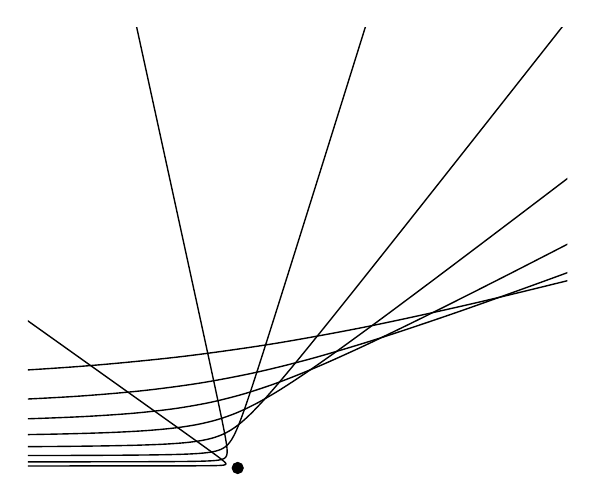
\begin{tikzpicture}[scale=1]
        %%% the logic
        % 1. draw the hyperbola (x-c)^2/a^2 - y^2/b^2 = 1 (the left branch)
        %    (x-c) means to align all focus
        % 2. rotate the hyperbola clockwise-ly such that the hyperbola
        %    is aligned on x axis, the rotation matrix is generated using
        %   [a  -b 
        %    b   a]/sqrt(a^2+b^2) 
        %    (think about why)
        %%%
        % limits & parameters
        \def\xa{-35}
        \def\xb{ 55}
        \def\ya{ -1}
        \def\yb{ 55}
        \def\tmax{4.5}
        \def\N{30} % number of points 
        \begin{axis}[ xmin=\xa,xmax=\xb,
                      ymin=\ya,ymax=\yb,
                      hide x axis, hide y axis,
                    ]
          \def\a{1}
          \foreach \u in {1,3,6,10,15,21,28,38}{
            \def\b{\u*0.25}
            \def\c{sqrt(\a^2+\b^2)}
            \addplot[line width=0.5,samples=\N,smooth,variable=\t,domain=-\tmax:\tmax]
               ({  \a/\c*(-\a*cosh(\t)-\c) + \b/\c*\b*sinh(\t) },
                { -\b/\c*(-\a*cosh(\t)-\c) + \a/\c*\b*sinh(\t) });
          } 
          \addplot[mark=*,mark size=2pt,mark options=solid] coordinates {(0,0)}; 
        \end{axis} 
      \end{tikzpicture}
      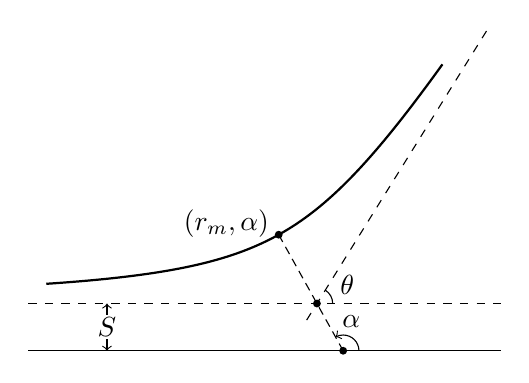
\begin{tikzpicture}
        \def\S{0.6}; % shift from center
        \def\a{1};
        \def\b{1.8};
        \draw (-4, 0) -- (2, 0);
        \draw[dashed] (-4, \S) -- (2, \S);
        \draw[<->] (-3, 0) -- node[fill=white,inner sep=1pt] {$S$} (-3, \S);
        \draw[thick,domain=-1.25:1.25,variable=\t,smooth,samples=300]
            plot(
                {( \a * (-\a*cosh(\t) - \S * (sqrt(\a^2+\b^2) / \b)) + \b * \b*sinh(\t)) / sqrt(\a^2 + \b^2)},
                {(-\b * (-\a*cosh(\t) - \S * (sqrt(\a^2+\b^2) / \b)) + \a * \b*sinh(\t)) / sqrt(\a^2 + \b^2)}
            );
        \draw[dashed,domain=-0.12:2,variable=\t,smooth,samples=20]
            plot(
                {( \a * (-\a*\a*\t - \S * (sqrt(\a^2+\b^2) / \b)) + \b * \b*\t) / sqrt(\a^2 + \b^2)},
                {(-\b * (-\a*\a*\t - \S * (sqrt(\a^2+\b^2) / \b)) + \a * \b*\t) / sqrt(\a^2 + \b^2)}
            );
        \node[circle,fill,inner sep=1pt] at (0, 0) {};
        \coordinate (P) at
            (
                {( \a * (-\a*cosh(0) - \S * (sqrt(\a^2+\b^2) / \b)) + \b * \b*sinh(0)) / sqrt(\a^2 + \b^2)},
                {(-\b * (-\a*cosh(0) - \S * (sqrt(\a^2+\b^2) / \b)) + \a * \b*sinh(0)) / sqrt(\a^2 + \b^2)}
            );
        \node[circle,fill,inner sep=1pt] at (P) {};
        \node[left,yshift=4pt] at (P) {$(r_m,\alpha)$};
        \draw[densely dashed] (P) -- (0, 0);
        \draw[->] (0.2, 0) arc (0:{atan(\a/\b)+90}:0.2) node[midway,above] {$\alpha$};
        \node[circle,fill,inner sep=1pt] at ({-\S*\a/\b}, \S) {};
        \draw ({-\S*\a/\b+0.2}, \S) arc (0:{180-2*atan(\b/\a)}:0.2)
            node[midway,right,yshift=4pt] {$\theta$};
      \end{tikzpicture}
      \tikzexternaldisable
\end{figure}
Question: how many particles will be scattered in the given solid
angle region (scattering cross section).
Let $V\sim 1/r$, $f\sim 1/r^2$.
Define the intensity of incident beam $I$
\begin{align*}
    I &= \text{\# of particles crossing a unit area perpendicular
    to the beam in unit time}
\end{align*}
The the number of particles scattered into $\d\Omega$
could be expressed as
\begin{align}
    \d N &= \sigma I \d \Omega,~
    \sigma = \frac{\d N}{I\d\Omega}
\end{align}
where $\sigma$ is called differential cross section,
which has the unit of area.

Particles in $[S,S+\d S]$ would be scattered into
$[\Omega, \Omega+\d\Omega]$, since $\d\Omega=2\pi\sin\theta\d\theta$
\begin{align}
    2\pi IS|\d S| &= \sigma I\d\Omega
    = 2\pi\sigma I\sin\theta|\d\theta|
    \Rightarrow
    \sigma = \frac{S|\d S|}{\sin\theta|\d\theta|}
\end{align}
The angular momentum of the incoming particles (wrt. to force center)
is
\begin{align}
    l &= mv_0 S = S\sqrt{2mE}
\end{align}
From the equation derived from central force problem
\begin{align}
    \alpha &= \int
    \frac{\d r}{r^2\sqrt{\frac{2mE}{l^2} - \frac{rmV}{l^2}-\frac{1}{r^2}}}
    \\
    &= \pi + \int_{-\infty}^{r_m}
    \frac{\d r}{r^2\sqrt{\frac{2mE}{l^2} - \frac{rmV}{l^2}-\frac{1}{r^2}}}
\end{align}
Let $r_m\equiv r_{\min}$ is the closest distance.
Define $\psi$ where
\begin{align}
    \alpha &= 
    \pi + \int_{-\infty}^{r_m}
    \frac{\d r}{r^2\sqrt{\frac{2mE}{l^2} - \frac{rmV}{l^2}-\frac{1}{r^2}}}
    = \pi - \psi
\end{align}
Hence $\theta=\pi-2\psi$.
Change the variable $u=1/r$, then
\begin{align}
    \psi &= 
    \int_0^{u_m=1/r_m}\frac{S\d u}{\sqrt{
        1 - \frac{V}{E} - S^2 u^2
    }}
\end{align}
Also note that
\begin{align}
    \sin\frac{\theta}{2} = \sin\frac{\pi-2\psi}{2} = \cos\psi = \frac{1}{\epsilon}
\end{align}
\begin{example}[Coulomb interaction]
Let 
\begin{align}
    f &= \frac{ZZ'e^2}{r^2},~
    V = \frac{ZZ'e^2}{r},~
    r = \frac{r_0}{1 + \epsilon\cos(\alpha-\alpha')}
\end{align}
choose $\alpha'=\pi$.
One can derive that
\begin{align}
    \epsilon &=
    \sqrt{1 + 
    \frac{2El^2}{m(ZZ'e^2)^2}}
    = \sqrt{ 1 + \left(
        \frac{2ES}{ZZ'e^2}
    \right)^2}
\end{align}
Using the trigonometric relationship between $\theta$ and $\epsilon$,
we have
\begin{align}
    S &= \frac{ZZ'e^2}{2E}\cot\frac{\theta}{2},~
    \left|\frac{\d S}{\d\theta}\right| = 
    \frac{ZZ'e^2}{4E}\frac{1}{\sin^2\frac{\theta}{2}}\\
    \Rightarrow
    \epsilon(\theta) &= 
    \left(\frac{ZZ'e^2}{4E}\right)^2 \frac{1}{\sin^4\frac{\theta}{2}}
\end{align}

\hl{check if $\alpha'=\pi$ or $\alpha'=\alpha_m$}
\end{example}


\newpage 
\section{Rigid Body}
\subsection{Coordinates of rigid body}
A rigid body is a system of point masses satisfying the constraint that
distance between any two points is a constant ($r_{ij}=\text{const}$
for all $i,j$).
Let $\mathbf{r}_i$, $\mathbf{r}_j$, and $\mathbf{r}_k$
be three points in the rigid body.
Let $\mathbf{r}_i$ has $3$ DOFs, 
since $r_ij$ is a constant, $\mathbf{r}_j$ has two DOFs.
Hence, $\mathbf{r}_k$ only have 1 DOFs.
The system has $3+2+1=6$ DOFs.

Or, alternatively, a rigid body has 3 coordinates for the origin of the coordinate
system fixed on the rigid body, and 3 angular variables to specify the orientation
of the rotated coordinate system.

\subsection{Orthogonal transformations}
Consider an orthogonal transformation $\mathbf{x}\mapsto\mathbf{x}'$
\begin{align}
    x_1' &= a_{11}x_1 + a_{12}x_2 + a_{13}x_3\\
    x_2' &= a_{21}x_1 + a_{22}x_2 + a_{23}x_3\\
    x_3' &= a_{31}x_1 + a_{32}x_2 + a_{33}x_3
\end{align}
Let $\mathbf{x}^2=\mathbf{x'}^2$, we have
\begin{align}
    \mathbf{x}^2 &= x_ix_i
    = x_i' x_i'
    = a_{ij}x_j a_{ik}x_k
    = \delta_{jk}x_jx_k
    = x_jx_j
    \Rightarrow
    a_{ij}a_{ik} = \delta_{jk}
\end{align}
This equation implies the orthogonal transformations have three DOFs.

Different views on rotational transformation
\begin{enumerate}
    \item Passive view the coordinate system is transformed
    \item Active view: the vector is transformed
\end{enumerate}

Consider two rotational matrix $A$ and $B$, let $C=AB$,
then 
\begin{align}
    C_{ij}C_{ik} &= A_{im}B_{mj}A_{in}B_{nk}
    = A_{im}A_{in}B_{mk}B_{nk}
    = \delta_{nm}B_{mj}B_{nk}
    = B_{nj}B_{nk}
    = \delta_{jk}
\end{align}
Non-commutative $AB\neq BA$.

Define the inverse transformation
\begin{align}
    x_i &= a'_{ij}x'_j = a'_{ij}a_{jk}x_k\Rightarrow
    a'_{ij}a_{jk} = \delta_{ik}
\end{align}
Note that
\begin{align}
    \left.
    \begin{aligned}
        \underbrace{a_{im}a_{ij}}_i a'_{jk} &= \delta_{mk}a'_{jk} = a'_{mk}\\
        a_{im}\underbrace{a_{ij}a'_{jk}}_j &= a_{im}\delta_{ik} = a_{km}
    \end{aligned}
    \right\}
    \Rightarrow a_{km} = a'_{mk}
\end{align}

\subsection{Euler angles}
A convenient choice of angle variables: Euler angles.
Steps:
\begin{enumerate}
    \item Rotate around $z$ axis by an angle $\phi$, rotational matrix $D$
    \item Rotate around $\xi$ axis by an angle $\theta$, rotational matrix $C$
    \item Rotate around $\xi'$ axis by an angle $\psi$, rotational matrix $B$
\end{enumerate}
We can always write any rotational matrix $A$ as $A = BCD$
Note that all rotations are rotations of \textbf{coordinate system}, which means,
$A$ is a change-of-basis matrix.
\begin{align}
    A &= 
    \begin{bmatrix}
        \cos\psi &  \sin\psi & 0\\
        -\sin\psi & \cos\psi & 0\\
        0 & 0 & 1
    \end{bmatrix}
    \begin{bmatrix}
        1 & 0 & 0\\
        0 & \cos\theta & \sin\theta \\
        0 & -\sin\theta & \cos\theta
    \end{bmatrix}
    \begin{bmatrix}
        \cos\phi & \sin\phi & 0\\
        -\sin\phi & \cos\phi & 0\\
        0 & 0 & 1
    \end{bmatrix}
\end{align}

\begin{figure}[htb]
    \tikzexternalenable
    \centering
    \tdplotsetmaincoords{60}{125}
    \tdseteulerzxz
    \begin{tikzpicture}[scale=3,tdplot_main_coords]
        \draw[canvas is yx plane at z=0,black!10!white,step=0.2] (0,0) grid (1,1);

        % first rotation
        \tdplotsetrotatedcoords{20}{0}{0}
        \draw[tdplot_rotated_coords,thick,-latex,blue] (0, 0, 0) -- (1, 0, 0) node[left]  {$\mathbf{N}$};
        \tdplotdrawarc{(0,0,0)}{0.35}{0}{20}{}{};
        \tdplotdrawarc[->]{(0,0,0)}{0.7}{0}{20}{anchor=north}{\tiny 1};
        \node at (0.5, 0.11, 0) {\footnotesize$\phi$};

        % second rotation
        \tdplotsetrotatedcoords{20}{20}{0}
        %\foreach \i in {0,...,17}{
        %    \tdplotsetrotatedthetaplanecoords{\i*10};
        %    \tdplotdrawarc[tdplot_rotated_coords]{(0,0,0)}{.35}{0}{360}{}{};
        %};
        \tdplotdrawarc[tdplot_rotated_coords]{(0,0,0)}{.2}{0}{20}{below}{\footnotesize$\psi$};
        \tdplotdrawarc[tdplot_rotated_coords,->]{(0,0,0)}{.6}{0}{20}{below}{\tiny 3};
        \tdplotsetrotatedthetaplanecoords{90};
        \tdplotdrawarc[tdplot_rotated_coords]{(0,0,0)}{.35}{0}{20}{above}{\footnotesize$\theta$};
        \tdplotdrawarc[tdplot_rotated_coords,<-]{(0,0,0)}{0.6}{0}{20}{anchor=south}{\tiny 2};

        % third rotation
        \tdplotsetrotatedcoords{20}{20}{20}
        \draw[tdplot_rotated_coords,thick,-latex,red] (0, 0, 0) -- (1, 0, 0) node[below]  {$x'$};
        \draw[tdplot_rotated_coords,thick,-latex,red] (0, 0, 0) -- (0, 1, 0) node[right] {$y'$};
        \draw[tdplot_rotated_coords,thick,-latex,red] (0, 0, 0) -- (0, 0, 1) node[right] {$z'$};

        % grid zy and xz
        \draw[canvas is zy plane at x=0,black!10!white,step=0.2] (0,0) grid (1,1);
        \draw[canvas is xz plane at y=0,black!10!white,step=0.2] (0,0) grid (1,1);

        % before rotation
        \draw[thick,-latex] (0, 0, 0) -- (1, 0, 0) node[left]  {$x$};
        \draw[thick,-latex] (0, 0, 0) -- (0, 1, 0) node[right] {$y$};
        \draw[thick,-latex] (0, 0, 0) -- (0, 0, 1) node[right] {$z$};
    \end{tikzpicture}    
    \tikzexternaldisable
\end{figure}

\begin{theorem}[Euler's theorem]
The general displacement of a rigid body with one point fixed is a rotation
around some axis $\mathbf{R}$.
Then
\begin{align}
    \mathbf{R}' &= A\mathbf{R} = \mathbf{R}
    \Rightarrow
    (A - I)\mathbf{R} = 0,~\det(A-I) = 0
\end{align}
\end{theorem}

Infinitesimal rotation transformation
\begin{align}
    \mathbf{x}' &= A\mathbf{x}
    = (1 + \epsilon) \mathbf{x}
    \Rightarrow
    x'_i = x_i + \epsilon_{ij}x_j
    = (\delta_{ij} + \epsilon_{ij})x_j
\end{align}
Hence
\begin{align}
    (\delta_{ki} + \epsilon'_{ki})x'_i &= 
    (\delta_{ki} + \epsilon'_{ki})
    (\delta_{ij} + \epsilon_{ij}) x_j
    = (\delta_{kj} + \epsilon'_{kj} + \epsilon_{kj} 
    + \epsilon'_{ki}\epsilon_{ij})x_j
    = x_k
\end{align}
Ignoring $\epsilon'_{ki}\epsilon_{ij}$ term,
we have $\epsilon'_{kj} = \epsilon^T_{jk} = -\epsilon_{kj}$,
given that $\epsilon$ is an antisymmetric matrix.
Let
\begin{align}
    \epsilon &= \begin{bmatrix}
        0 & -d\Omega_3 & \d\Omega_2\\
        \d\Omega_3 & 0 & -\d\Omega_1\\
        -\d\Omega_2 & \d\Omega_1 & 0
    \end{bmatrix},~
    \boldsymbol{\Omega} = \begin{bmatrix}
        \Omega_1\\ \Omega_2 \\ \Omega_3
    \end{bmatrix}
\end{align}
Then
\begin{align}
    \d\mathbf{x} &= \epsilon\mathbf{x} = \d\boldsymbol{\Omega}\times\mathbf{x}
\end{align}

\subsection{Rate of change of a vector}
Let $\mathbf{R}$ be one point inside the rigid body, then
the motion can be decomposed into rotational motion of the
body coordinate and the translational motion of the body
\begin{align}
    \left(\frac{\d\mathbf{R}}{\d t}\right)_\text{space}
    &= \left(\frac{\d\mathbf{R}}{\d t}\right)_\text{body}
    + \frac{\d\boldsymbol{\Omega}}{\d t}\times\mathbf{R}\\
    \Rightarrow
    \mathbf{V}_\text{space} &= \mathbf{V}_\text{body}
    + \boldsymbol{\omega}\times\mathbf{R}
    \label{eq:rigidV}
\end{align}
Decompose $\boldsymbol{\omega}$ into unit vectors corresponds
to Euler angles and the body coordinate
\begin{align}
    \boldsymbol{\omega} &= 
    \dot\phi e_\phi + \dot\theta e_\theta + \dot\psi e_\psi
    = \omega_{x'}\mathbf{i}' + \omega_{y'}\mathbf{j}'
    + \omega_{z'}\mathbf{k}'
\end{align}
From the figure we can find that
\begin{align}
    e_\phi &= \mathbf{k}
    = \sin\theta\sin\psi\mathbf{i}' + \sin\theta\cos\psi\mathbf{j}'
    + \cos\theta\mathbf{k}'\\
    e_\theta &= \cos\psi\mathbf{i}' - \sin\psi\mathbf{j}'\\
    e_\psi &= \mathbf{k}'
\end{align}
Hence
\begin{align}
    \omega_{x'} &= \dot\phi\sin\theta\sin\psi + \dot\theta\cos\psi\\
    \omega_{y'} &= \dot\phi\sin\theta\cos\psi - \dot\theta\sin\psi\\
    \omega_{z'} &= \dot\psi + \dot\phi\cos\theta
\end{align}

\subsection{The Coriolis effect}
From equation \ref{eq:rigidV} we have
\begin{align}
    \mathbf{a}_\text{space} &=
    \mathbf{a}_\text{body}  + \boldsymbol{\omega}\times\mathbf{V}_\text{\space}\\
    \Rightarrow
    m\mathbf{a}_\text{body} &= 
    \mathbf{F} - 2m\boldsymbol{\omega}\times\mathbf{V}_\text{body}
    - m\boldsymbol{\omega}\times(\boldsymbol{\omega}\times\mathbf{R})
\end{align}
The term $-2m\boldsymbol{\omega}\times\mathbf{V}_\text{body}$
is the Coriolis force.

\newpage
\section{EOM of rigid body}
\subsection{Angular momentum and kinetic energy}
It is often convenient to choose the COM of the rigid body as the origin
of the body system.
Suppose the motion only involves rotation, the angular momentum is
\begin{align}
    \mathbf{L} &= 
    \sum_i m_i (\mathbf{r}_i\times\mathbf{v}_i)
    = \sum_i m_i [\mathbf{r}_i\times(\symbfit{\omega}\times\mathbf{r}_i)]
    = \sum_i m_i[\mathbf{r}_i^2\symbfit{\omega} - \mathbf{r_i}(\mathbf{r}_i
    \cdot\symbfit{\omega})]
\end{align}
Consider the components of the equation
\begin{align}
    L_x &= \sum_i m_i[\omega_x(\mathbf{r}_i^2 - x_i^2) - \omega_yx_iy_i-\omega_z x_iz_i]\\
    L_y &= \sum_i m_i[\omega_y(\mathbf{r}_i^2 - y_i^2) - \omega_xx_iy_i-\omega_z y_iz_i]\\
    L_z &= \sum_i m_i[\omega_x(\mathbf{r}_i^2 - z_i^2) - \omega_xx_iy_i-\omega_y y_iz_i]\\
    \Rightarrow
    \begin{bmatrix}
        L_x\\L_y\\L_z
    \end{bmatrix} &=
    \begin{bmatrix}
        I_{xx} & I_{xy} & I_{xz}\\
        I_{yx} & I_{yy} & I_{yz}\\
        I_{zx} & I_{zy} & I_{zz}
    \end{bmatrix}
    \begin{bmatrix}
        \omega_x\\ \omega_y\\ \omega_z
    \end{bmatrix}
\end{align}
Written the equation in the integral form
\begin{align}
    I_{ij} &= 
    \int_V\rho(\mathbf{r})\d\mathbf{r}\ (\mathbf{r}^2\delta_{ij} - r_ir_j)
\end{align}
The total kinetic energy is
\begin{align}
    T 
    &= \sum_i \frac{1}{2}m_i\mathbf{v}_i^2
    = \sum_i \frac{1}{2}m_i(\symbfit{\omega}\times\mathbf{r}_i)\cdot\mathbf{v}_i
    = \frac{1}{2}\symbfit{\omega}\cdot\sum_i m_i(\mathbf{r}_i\times\mathbf{v}_i)
    = \frac{1}{2}\symbfit{\omega}\cdot\mathbf{L}
    = \frac{1}{2}\symbfit{\omega}^T I\symbfit{\omega}
    = \frac{1}{2}I_{ij}\omega_i\omega_j
\end{align}
If $\symbfit{\omega}=\omega\mathbf{n}$, then
\begin{align}
    T &= \frac{1}{2}\omega^2\mathbf{n}^TI\mathbf{n}
\end{align}
If there is a translational motion
\begin{align}
    \mathbf{v}_i &= \mathbf{v}_0 + \symbfit{\omega}\times\mathbf{r}_i\\
    \mathbf{r}_i &= \mathbf{r}_0 + \mathbf{r}_i'\\
    \Rightarrow\mathbf{L}
    &= \sum_i(\mathbf{r}_0+\mathbf{r}_i')\times(\mathbf{v}_0 + \symbfit{\omega}
    \times\mathbf{r}_i)
    = M\mathbf{r}_0\times\mathbf{v}_0 
    + \sum_i m_i\mathbf{r}_i'\times(\symbfit{\omega}\times\mathbf{r}_i')
\end{align}
Hence, the kinetic energy becomes
(let $\symbfit{\omega}=\omega\mathbf{n}$)
\begin{align}
    T &= \sum_i \frac{1}{2}m_i(\mathbf{v}_0 + \symbfit{\omega}\times\mathbf{r}_i)^2
    = \sum_i \frac{1}{2}m_i\mathbf{v}_0^2 + m_i\mathbf{v}_0\cdot
    (\symbfit{\omega}\times\mathbf{r}_i)
    + \frac{1}{2}\omega^2m_i(\mathbf{n}\times\mathbf{r}_i)^2
    = \frac{1}{2}M\mathbf{v}_0^2 + \frac{1}{2}I\omega^2
\end{align}

Angular momentum around any point
\begin{align}
    I_a &= \sum_i m_i(\mathbf{n}\times\mathbf{r}_i)^2
    = \sum_i m_i[\mathbf{n}\times(\mathbf{R} + \mathbf{r}_i')]^2
    = \sum_i m_i(\mathbf{n}\times\mathbf{R})^2 + \sum_i m_i(\mathbf{n}\times
    \mathbf{r}_i')^2
    = M(\mathbf{n}\times\mathbf{R})^2 + I_\text{COM}
\end{align}

\subsection{The eigenvalues of the inertia tensor}
We can diagonalize the matrix $I$ s.t.
\begin{align}
    I &= \begin{bmatrix}
        I_1 & & \\
        & I_2 & \\
        & & I_3
    \end{bmatrix}
\end{align}
The diagonal terms are called the principle moments of inertia,
and the axes that diagonalize the matrix are called the
principal axes.


% \end{multicols*}
\end{document}

